\section{Elméleti háttér}

\subsection{A jármű kinematikai modellje}

Mielőtt a használt A* algoritmus útvonalat tudna keresni, fontos megismerni az algoritmus álltal használt gráfcsúcsok adatainak elméleti hátterét. Ezt egy kinematikai egypályás modellel (később STM) reprezentáljuk, aminek a lényege, hogy lefedje a jármű $x$ és $y$ koordinátáját a koordinátarendszerben, valamint a jármű orientációját ($\theta$). Ezek segítségével kapjuk a következő modellt \cite{kug_obp}:
\begin{align}
    x' &=v\cos(\theta) \\
    y' &=v\sin(\theta) \\
    \theta' &=\frac{v}{L}\tan(\delta)
\end{align}

Az első két egyenlet a jármű sebességét ($v$) bontja $x$ és $y$ irányú komponensekre, a harmadik egynelet pedig a jármű orientációjának változását írja le a kormányzott kerekek állásának szöge ($\delta$) és a tengelyhossz ($L$) függvényében. Mind $v$ és $\delta$ bemeneti adatok, csak $L$ paraméter az egyenletrendszerben. \\
Az előző egyenletrendszerben viszont nem szerepelt korlátozás a kormányzott kerekek szögének változására, tehát matematikailag lehetséges lenne az ugrásszerű változás is. Hogy ezt elkerüljük, a kerekek szögét ($\delta$) is bevezetjük, mint állapot és helyette a kerékállások változásának a szögsebessége ($v_\delta$) lesz a második bemeneti adat. Tehát a végső modell:
\begin{align}
    x' &=v\cos(\theta) \\
    y' &=v\sin(\theta) \\
    \theta' &=\frac{v}{L}\tan(\delta) \\
    \delta' &=v_\delta
\end{align}

\begin{figure}[H]
	\centering
	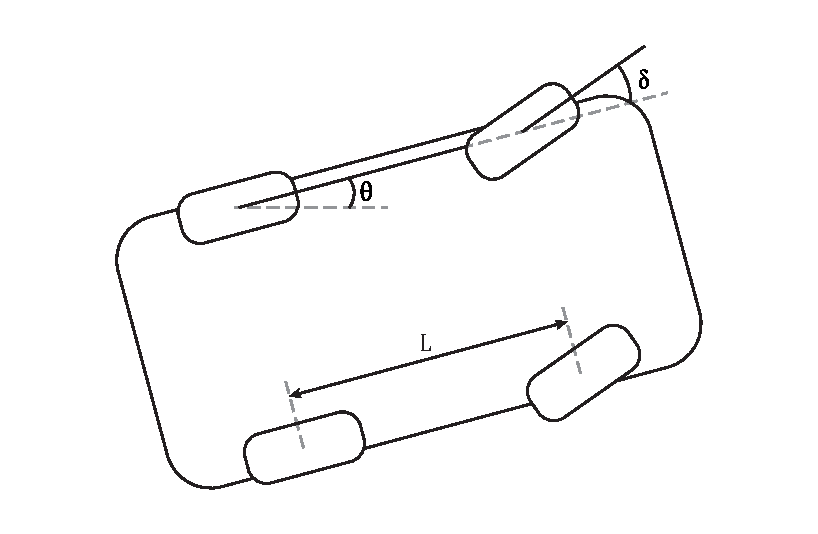
\includegraphics[width=300px]{stm_graphic}
	\caption{Az STM geometriai vizualizációja}
	\label{fig:STMdrawing}
\end{figure}

Az $[x, y, \theta, \delta]^T$ négyest a forráskódban a
{\fontfamily{cmtt}\selectfont rbp::pp::common::CPosture} osztály reprezentálja, amely \az\told{\ref{src:CPostureClass}}+as{} kódrészletben látható.

\begin{note}
A (\ref{src:CPostureClass}) osztályhoz hasonlóan léteznek a benne szereplő {\fontfamily{cmtt}\selectfont rbp::pp::common::CPose} ($[x, y, \theta]^T$) és az azon belüli {\fontfamily{cmtt}\selectfont rbp::pp::common::CPosition} ($[x, y]^T$) osztályok is. A \emph{getter} és \emph{setter} függvények helymegtakarítás miatt nincsenek megjelenítve, intuitívan állítható és lekérdezhető az $x, y, \theta, \delta$ paraméter ($x, y, \theta$ egyben is mint {\fontfamily{cmtt}\selectfont CPose} és $x, y$ mint {\fontfamily{cmtt}\selectfont CPosition}).
\end{note}
\clearpage

\lstset{caption={A CPosture osztály kivonata}, label=src:CPostureClass}
\begin{lstlisting}[language={C++}]
#include "rbp/pp/common/common_pose.hpp"

namespace rbp::pp::common
{

class CPosture
{
public:
    CPosture() = default;

    CPosture(const Real x, const Real y, const Real yaw, const Real curvature)
        : m_pose{x, y, yaw}
        , m_curvature{Curvature(curvature)} {}

    CPosture(const CPosition& position, const Real yaw, const Real curvature)
        : m_pose{position, yaw}
        , m_curvature{Curvature(curvature)} {}

    CPosture(const CPose& pose, const Real curvature)
        : m_pose{pose}
        , m_curvature{Curvature(curvature)} {}

    // getters, setters
    // ...
private:
    CPose     m_pose;
    Curvature m_curvature;
};
\end{lstlisting}

\subsection{Együttműködés az A* algoritmussal}

A következő feladat, hogy az A* gráfkeresését és az előző alfejezetben tárgyalt kinematikai modellel leírt járművek útkeresési problémáját valamilyen formában kombináljuk. A szoftverben ez a \emph{"state lattice"} megközelítéssel van megvalósítva. Ennek a módszernek a lényege, hogy a rendelkezésre álló teret (vagy egy részét) előre diszkrét állapotokra osztja. Ezeket az állapotokat pedig valamilyen hálón elhelyezi, ahol a szomszédos állapotok előre definiált mozgással érhetőek el \cite{statelattice}.
Az így definiált állapotokat már használhatjuk az A* algoritmus gráfjának csúcsaiként, de a szomszédos csúcsokat élekkel még nem köthetjük össze. Ezeket az előre definiált mozgások kötik össze (\emph{Motion Primitives} \cite{kinodyno_motionprimitives}), melyeket diszkretizálni lehet, hogy a valódi útvonal kellően precíz pontjait megkapjuk.
Sok lehetőség van a \emph{Motion Primitive-ek} megválasztására, de az útvonaltervezéshez gyakran használt csoport is létezik. Ezek a kormányzási függvények \cite{reeds-shepp}, melyek alap görbéket
írnak le, mint teljes jobb illetve bal kanyar, vagy egyenes. Ezek a függvények jó választások a feladathoz, hiszen könnyen definiálhatók a jármű minimális sugarú fordulási körével.

\begin{note}
A valós algoritmusban nem csak ezeket a \emph{Motion Primitive-eket} használjuk. Ennek az oka, hogy a végleges STM-nek $\delta$-ban folytonosnak kell lennie. A fent említett egyszerű kormányzási függvényeket klotoidokkal \cite{clohtoids} kötjük össze, hogy a folytonosságnak eleget tegyen az útvonal.
\end{note}

\begin{figure}[H]
    \centering
	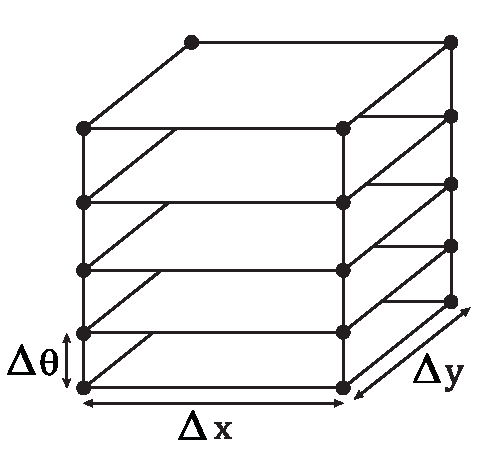
\includegraphics[width=240px]{state_lattice_graphic}
	\caption{A \emph{state lattice} modell egy kis részének diszkretizációja}
	\label{fig:stateLatticeDrawing}
\end{figure}

\begin{explain}
    \Az\told{\ref{fig:stateLatticeDrawing}}+as{} ábrán látható formális paraméterekkel jelölve a diszkretizáció. Ezen paraméterek segítségével egy háromdimenziós térként lehet vizualizálni a \emph{state lattice-t}. Ha a járművet $x$ vagy $y$ irányba mozgatjuk, akkor annak megfelelően az $(x, y)$ síkon mozog. Mivel a járművet a hátsó tengelyének középpontjával tudjuk elhelyezni, a $\theta$ irányú forgatás nem lenne látható. Ezt a problémát oldja meg a harmadik dimenzió, így minden diszkrét $\Delta \theta$ értékhez tartozik egy $(x, y)$ sík. Ezen paraméterek értéke előre meghatározott, például $\Delta x=\Delta y =3cm, \Delta \theta=1$°.
\end{explain}

\subsection{A részekre osztott útvonaltervezés}

Mivel az útvonaltervezőben már adott volt a két pont közti útvonal tervezésének lehetősége, a nagyobb kérdés az maradt, hogy hogyan lehet köztes pontokat meghatározni, amik segítik a jármű haladását és nem teszik sokkal hosszabbá a kapott utat. Ezt a problémát referencia konfigurációk \cite{kug_obp} (később RC) generálásával oldottam meg. Ezek a $[x, y, \theta]^T$ hármasok olyan \emph{state lattice} beli pontok, amelyekhez egy megadott pontból egy egyszerű mozdulat segítségével jutunk. Persze ez a feladat csak akkor "egyszerű" igazán, ha nincsenek akadályok a megadott pont és az RC közt. Ezért az RC-nek nem kell elérhetőnek lennie, és a hozzá vezető útnak sem kell, hogy ütközésmentesen végigjárható legyen. Minden $q_L$ ponthoz (\emph{Landmark}) kettő darab RC generálódik, egy párhuzamos ($q_{RC_P}$) és egy merőleges ($q_{RC_O}$). A két RC a következőképpen írható le:
\begin{align}
    q_{RC_P} &= q_L + 
    \begin{bmatrix}
        \Delta x + \sigma _{xP}\\
        \sigma _{yP}\\
        \sigma _{\theta P}
    \end{bmatrix}\\
    q_{RC_O} &= q_L +
    \begin{bmatrix}
        \Delta x + \sigma _{xO}\\
        \sigma _{yO}\\
        \pm \frac{\pi}{2} + \sigma _{\theta O}
    \end{bmatrix}
\end{align}

Az egyenletben szereplő $\Delta x$ és $\sigma$ paraméterek, amivel a felhasználó személyre szabhatja, hogy hogyan generálódjanak az RC-k. A $\Delta x$ paraméter mondja meg, hogy a járműnek minimum mekkora utat kell megtennie $x$ irányba. A $\sigma$ pedig leírja, hogy a minimális mozgáson felül a három irányba még mennyit haladjon a jármű. Minden $x, y, \theta$ és $P, O$ paraméterhez más $\sigma$ érték tartozik. Például $\sigma _{yP}$ és $\sigma _{yO}$ nagyban eltérnek egymástól, hiszen a merőleges parkoláshoz tartozó nagyobb $\theta$ változást csak nagyobb távon lehet egyszerűen végrehajtani. Ehhez a $\theta$ paraméter és merőleges RC esetén még hozzáadódik $\pm \frac{\pi}{2}$ is attól függően, hogy melyik fordulás van közelebb a cél konfigurációhoz. Az értékek vizualizációja \az\told{\ref{fig:RCDrawing}}+as{} ábrán látható.
\begin{note}
Ideális esetben minden $\sigma$ paraméter egy adott pontosságú intervallum lenne, amiből véletlenszerűen választhatnánk értéket minden RC generálásakor. Ezzel az útvonaltervezőt még jobban tudjuk kényszeríteni, hogy fedezze fel a rendelkezésre álló teret. Mivel beágyazott szoftverben nem előnyös és nehezen megvalósítható (az ipar szabályain belül) a véletlenszámok használata, ezért minden ilyen paraméter egy egyszerű szám, ami járművenként állítható. Az RC-ket a forráskódban ugyanúgy a {\fontfamily{cmtt}\selectfont rbp::pp::common::CPose} osztály valósítja meg, mint a \emph{state lattice} többi pontját.
\end{note}

\begin{figure}[H]
    \centering
	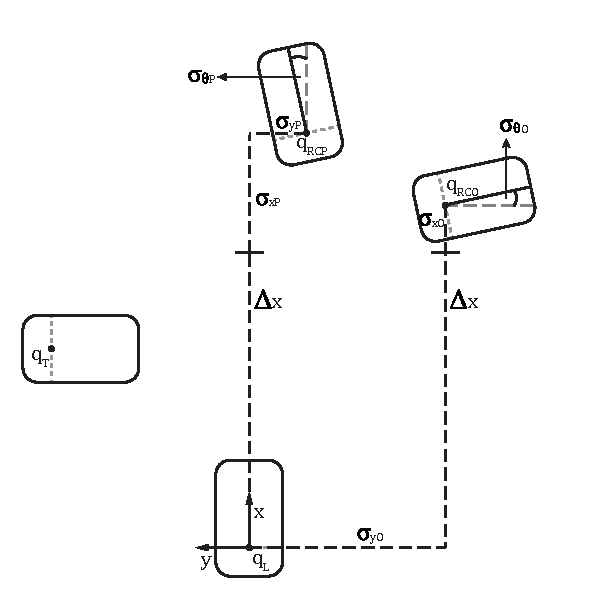
\includegraphics[width=350px]{rc_graphic}
	\caption{$q_L$-hez tartozó $q_{RC_P}$ és $q_{RC_O}$ konfigurációk}
	\label{fig:RCDrawing}
\end{figure}
\clearpage